\section{Synthesis from K-Inductive Proofs of Realizability}
\label{sec:kinductionsynth}
In this section we %define Assume-Guarantee contracts (Sect.~\ref{sec:pre}),
 sketch an existing algorithm for determining contract realizability
(Sect.~\ref{sec:old}), present our new algorithm that bridges the gap between the realizability checking and synthesis (Sect.~\ref{sec:realizability-synthesis}),
and finally illustrate how the algorithm works on an example
(Sect.~\ref{sec:example}).

\iffalse
\subsection{Assume-Guarantee Contracts}
\label{sec:pre}

One popular way to describe software requirements is through Assume-Guarantee
contracts, where requirements are expressed using safety properties that are
split into two categories, \emph{assumptions} and \emph{guarantees}.
Contract \emph{assumptions} are properties that restrict the set of valid inputs
a system can process, while \emph{guarantees} dictate system behavior by constraining system outputs.

For example, consider the contract with the assumption $A = \{x\neq
y\}$ and the guarantee $G = \{x \leq y \Longrightarrow z =
\textit{true}, x \geq y \Longrightarrow z = \textit{false}\}$, for a component with two inputs $x$ and $y$ and one output $z$.  By assumption, $x \neq y$, so the implemented system could set $z$ to true if $x < y$ and false otherwise. Of course, multiple implementations may exist for the same contract. An
alternative approach, for example, could set $z$ to false if $x > y$, and true
otherwise. Determining whether an implementation can be constructed to satisfy
the contract for all possible input sequences is the \emph{realizability} problem, while automatically constructing a witness of the proof of realizability of the contract is the \emph{program synthesis} problem.  The contract $(A,G)$ above is obviously \emph{realizable}, and therefore an implementation can be constructed.
However, if the assumption is omitted then the contract is \emph{unrealizable}, since there is no correct value for $z$ when $x=y$.

We describe a system using the disjoint sets $state$ and $inputs$.
Formally, an \emph{implementation} is a \emph{transition system}
described by an initial state predicate $I(s)$ of type $state \to
bool$ and by a transition relation $T(s,i,s')$ of type $state \to
inputs \to state \to bool$.

An Assume-Guarantee (AG) contract can be formally defined by a set of
\emph{assumptions} and a set of \emph{guarantees}. The
\emph{assumptions}, $A: state \rightarrow inputs \rightarrow bool$,
impose constraints over the inputs which may be modal in terms of the
previous state. The \emph{guarantees} $G$ consist of two separate
subsets $G_I: state \rightarrow bool$ and $G_T: state \rightarrow
inputs \rightarrow state \rightarrow bool$, where $G_I$ defines the
set of valid initial states, and $G_T$ specifies the properties that
need to be met during each new transition between two states. Note
that we do not necessarily expect that a contract would be defined
over all variables in the transition system, but we do not make any
distinction between internal state variables and outputs in the
formalism. This way, we can use state variables to (in some cases)
simplify the specification of guarantees.
\fi
%\vspace{-.5em}
\subsection{Realizability of Contracts}
\label{sec:old}
%\vspace{-.5em}

The synthesis algorithm proposed in this paper is built on top of our previous work on a realizability checking algorithm~\cite{gacek2015towards}. The coinductive notion of viable states described in Def.~\ref{eq:viable} is not useful to determine realizability in practice, and as such we have to use an approximation. With that in mind, we express the problem of realizability using the description of a state being \emph{extendable after n steps}, if any valid path of length $n-1$ starting from $s$ can be extended in response to any valid input:

%\begin{definition*}
%\label{def:extend}
%A state $s$ is extendable after $n$ steps, denoted $\mathit{Extend}_{n}(s)$, if
%any valid path of length $n-1$ starting from $s$ can be extended in response to
%any valid input.%
%
%\begin{equation}
\begin{multline}%
%\mathit{Extend}_{n}(s)
\extendable \triangleq \forall i_1, s_1, \ldots, i_n, s_n.\\ A(s, i_1) \land G_T(s, i_1, s_1)
\land \cdots \land
A(s_{n-1}, i_n) \land G_T(s_{n-1}, i_n, s_n)
\implies \\
\forall i.~ A(s_n, i) \implies \exists s'.~ G_T(s_n, i, s')
\label{def:extend}
\end{multline}
%\end{definition*}
%\end{equation}

The algorithm for realizability uses Def.~\ref{def:extend} in two
separate checks that correspond to the two traditional cases exercised
in k-induction. Initially, it is proved that the set of initial states is
not empty, by checking for the existence of at least one
state that satisfies $G_I$. For $\basecheck(n)$, we ensure
that all initial states are extendable for any path of length $k < n$,
while the inductive step of $\extendcheck(n)$ tries to prove that
all valid states are extendable for any path of length $n$. Therefore,
we attempt to find the smallest $n$, for which the two following
$\forall\exists$-formulas are valid:%
%
\begin{equation}
\label{eq:sbcheck}
\basecheck(n) \triangleq \forall k < n. (\forall s. G_I(s)
	  	\implies \extendablek)
\end{equation}%
%
\begin{equation}
\label{eq:echeck}
\extendcheck(n) \triangleq \forall s. \extendable
\end{equation}

The realizability checking algorithm has been used to effectively find cases
where the traditional consistency check (i.e. the existence of an assignment
to the input variables for which the output variables satisfy the contract)
failed to detect conflicts between stated requirements in case studies of
different complexity and importance. It has also been formally verified using the Coq proof assistant in terms of its
soundness, for the cases where it reports that a contract is
realizable~\cite{katis2015machine}.

\subsection{Program Synthesis from Proofs of Realizability}
\label{sec:realizability-synthesis}

%While the implemented algorithm on realizability provided us with meaningful
%results during the verification of several contracts,
%The main contribution of the paper is an algorithm for deriving implementations from the proof of a contract's realizability.
%Indeed, t
The algorithm sketched in Sect.~\ref{sec:old} can be further used for solving the more complex problem of
\emph{program synthesis} to automatically derive an implementation from the proof of a contract's realizability. 
%That is, we can automatically
%derive implementations from the proof of a contract's realizability.
%The limited power of SMT solvers
%in terms of solving formulas containing nested quantifiers immediately ruled
%out the prospect of using one as our primary synthesis tool. Fortunately,
%we are able to exploit our prior results in the scope of solving validity and
%Skolemizing $\forall\exists$-formulas (to be described in Sect.~\ref{sec:aeval}).
%The idea is simple.
Consider checks~\eqref{eq:sbcheck}
and~\eqref{eq:echeck} that are used in the realizability checking
algorithm. Both checks require that the reachable states explored are
extendable using Def.~\ref{def:extend}. The key insights are then 1)
we can start with a arbitrary state in $G_I$ since it is non-empty, 2)
we can use witnesses from the proofs of $\extendablek$ in
$\basecheck(n)$ to create a valid path of length $n-1$, and 3) we
can extend that path to arbitrary length by repeatedly using the
witness of the proof of $\extendable$ in
$\extendcheck(n)$.

In first order logic, witnesses for valid $\forall\exists$-formulas
are represented by Skolem functions. Intuitively, a Skolem function
expresses a connection between all universally quantified variables in
the left-hand side of the $\forall\exists$-formulas~\eqref{eq:sbcheck}
and~\eqref{eq:echeck} and the existentially quantified variable $s'$
within $\extendable$ \andreas{changed from ``$\mathit{Extend}$''} on the right-hand side. We generate Skolem functions from the validity of~\eqref{eq:sbcheck} and~\eqref{eq:echeck} using the \aeval tool~\cite{fedyukovich2015automated}. We refer the reader to Sect.~\ref{sec:aeval} for a brief description of its functionality.\andreas{We need to discuss whether we will have a dedicated \aeval section in the journal, as the space is quite limited.}

%Our algorithm uses the \aeval tool, detailed in Sect.~\ref{sec:aeval} \andreas{we need to discuss whether a dedicated section on \aeval is necessary for this paper, as the space is limited}
%, to generate such Skolem functions from the validity of~\eqref{eq:sbcheck} and~\eqref{eq:echeck}.

%\synthesisalgorithm

%% During the k-induction algorithm, two parallel
%% engines (\textsc{BaseEngine, ExtendEngine}) handle the base and
%% inductive step checks of validity of $\forall\exists$-formulas.
%% The proof of a formula's validity is closely tied to the process of
%% Skolemization: for every step that \textit{BaseCheck(n)} is valid,
%% \aeval provides a Skolem function to witness that validity.


\begin{figure}
\scalebox{.85}{
\begin{minipage}{0.65\textwidth}
\begin{algorithm}[H]
\caption{\jsyn (A : assumptions, G : guarantees)}
\label{alg:kindsynthesis}
\begin{algorithmic}[1]
	\State $Skolems \gets \langle \rangle$;%\Comment{List of Skolem Functions}
	\State $InitResult \gets $\textsc{Sat?}$(G_I)$;
	\If{$(\isUnsat(InitResult))$}
		\Return \unrealizable, $\emptyset$, $\langle \rangle$;
	\EndIf
	\For{$(i \gets 0; \mathbf{true}; i \gets i + 1)$}
		\State $\tuple{\mathit{valid}, \skolems} \gets \aeval(\extendcheck(i))$
%		\State $ExtendResult \gets \aeval(ExtendCheck(i))$;
		%\If{$(\isValid(ExtendResult))$}
		\If{$\mathit{valid}$}
			\State $Skolems.Add(\skolems)$
			%\State $Skolems.Add(ExtendResult.Skolem)$;
			\Return \realizable, $Skolems$;
		\EndIf
		\State $\tuple{\mathit{valid}, \skolems} \gets \aeval(\basecheck_{k}(i))$
		%\State $BaseResult \gets \textsc{\aeval}(BaseCheck_{k}(i))$;
		%\If{$(\isInvalid(BaseResult))$}
		\If{$\lnot \mathit{valid}$}
			\Return \unrealizable, $\emptyset$, $\langle \rangle$;
		\EndIf
		\State $Skolems.Add(\skolems)$
		%\State $Skolems.Add(BaseResult.Skolem)$;
	\EndFor
\end{algorithmic}
\end{algorithm}
\end{minipage}
}
\hspace{1cm}
\scalebox{.8}{
\begin{minipage}{0.38\textwidth}
\setcounter{algorithm}{0}
\begin{template}[H]
\caption{Structure of an implementation}
\label{alg:synt}
\begin{algorithmic}[1]
	\State $\textsc{assign\_Init()}$;
	\State $\textsc{read\_inputs()}$; 		
	\State $\textsc{Skolems}[0]()$;
  	\State $\ldots$
  	\State $\textsc{read\_inputs()}$;
  	\State $\textsc{Skolems}[k-1]()$;
	\While{true}
 		\State $\textsc{read\_inputs()}$;
 		\State $\textsc{Skolems}[k]()$;
 		\State $\textsc{update\_history()}$;
	\EndWhile
\end{algorithmic}
\end{template}
\end{minipage}
}
\end{figure}

Alg.~\ref{alg:kindsynthesis} named \jsyn provides a summary of the synthesis
procedure. The algorithm first determines whether the set of initial states $G_I$ is non-empty.
Second, it attempts to construct an inductive proof of the system's
realizability, using \aeval\ to find Skolem witnesses. For each call of \aeval we write $\tuple{x, y} \gets \aeval(\ldots)$: $x$ specifies if the given formula is valid or not, and $y$ contains the Skolem function (only in case of the validity). The algorithm iteratively proves $\mathit{BaseCheck_k(i)} \triangleq \forall s. G_I(s) \implies \mathit{Extend}_i(s)$ and accumulates the resulting Skolem functions. If $\mathit{BaseCheck_k(i)}$ ever fails, we know $\mathit{BaseCheck(i)}$ would also fail and so the system is unrealizable. At the same time, the algorithm tries to prove $\mathit{ExtendCheck(i)}$. As soon as the inductive step of $\mathit{ExtendCheck(i)}$ passes, we have a complete k-inductive proof stating that the contract is realizable. We then complete our synthesis procedure by generating a Skolem function that
corresponds to the inductive step, and return the list of the Skolem functions.  Note that in Alg.~\ref{alg:kindsynthesis} for a particular depth $k$, we perform the extends check prior to the base check. The intuition is that $\mathit{BaseCheck(i)}$ checks $\forall k < i$; thus, it is one step ``smaller'' than the extends check and this avoids a special case at $k=0$.

Given a list of Skolem functions, it remains to plug them into
an implementation skeleton as shown in Template~\ref{alg:synt}.
The combination of Lustre models and k-inductive proofs
allow the properties in the model to manipulate the
 values of variables up to $k-1$ steps in the past. Thus,
the first step of an implementation  (method \textsc{assign\_Init()})
 creates an array for each state variable of size $k+1$, where
$k$ is the depth of the solution to Alg.~\ref{alg:kindsynthesis}.
This array represents the depth of history necessary to compute
the recurrent Skolem function produced by the $\extendcheck(n)$ process.
The $\basecheck(n)$ Skolem functions initialize this history.

In each array, the $i$-th element, with $0\leq i \leq k-1$,
corresponds to the value assigned to the variable after the call to
$i$-th Skolem function. As such, the first $k-1$ elements of each array
correspond to the $k-1$ Skolem functions produced by the
$\basecheck(n)$ process, while the last element is used by the
Skolem function generated from the formula corresponding to the
$\extendcheck(n)$ process.

The template uses the Skolem functions generated by \aeval for each
of the $\basecheck(n)$ instances to describe the initial behavior of
the implementation prior to depth $k$.  %\textcolor{red}{This process starts
% from the memory-free witness $\init$ to the initial guarantee $G_I$, which is
%assigned in method \textsc{assign\_Init()}}.
There are two ``helper'' operations:
\textsc{update\_history()} shifts each element in the arrays one position
forward (the 0-th value is simply forgotten), and \textsc{read\_inputs()} reads the
current values of inputs into the $i$-th element of the variable arrays,
where $i$ represents the $i$-th step of the process.
Once the history is entirely initialized using the $\basecheck(n)$ Skolem functions,
we add the Skolem function for the $\extendcheck(n)$ instance to describe the
recurrent behavior of the implementation (i.e., the next value of outputs in
each iteration in the infinite loop).

To establish the correctness of the algorithm,
we have constructed machine-checked proofs as to the validity of $\mathit{BaseCheck(n)}$ and
$\mathit{ExtendCheck(n)}$ using the Skolem functions.
The entirety of the models explored in
this paper only involved proofs of realizability of length $k$ equal to 0 or
1.
As such, we limited our proofs of soundness to these two specific cases. We will
extend the proofs to capture any arbitrary $k$ as part of our future work.
The theorems were written and proved using the Coq proof
assistant.~\footnote{The proofs can be found
at~\href{https://github.com/andrewkatis/Coq}{https://github.com/andrewkatis/Coq}}.

\begin{theorem}[Bounded Soundness of BaseCheck and ExtendCheck using Skolem Functions]
Let $\basecheck_{S(s_n,i,s')}(n)$ and $\extendcheck_{S(s_n,i,s')}(n)$, $n \in {0,1}$, be the valid variations of the corresponding formulas $\mathit{BaseCheck(n)}$ and $\mathit{ExtendCheck(n)}$, where the existentially quantified part $\exists s'.~G_T(s_n, i, s')$ has been substituted with a witnessing Skolem function
$S(s_n,i,s')$.  We have that:
\begin{itemize}
\item $\forall (A,G_{I},G_{T}). \mathit{BaseCheck}(n) \Rightarrow \mathit{BaseCheck}_{S(s_n,i,s')}(n)$
\item $\forall (A,G_{I},G_{T}). \mathit{ExtendCheck}(n) \Rightarrow
ExtendCheck_{S(s_n,i,s')}(n)$
\end{itemize}
\end{theorem}
\begin{proof}
The proof uses the definition $\mathit{Extend}_n(s)$ of an extendable state,
after replacing the next-step states with corresponding Skolem functions. From there,
the proof of the two implications is straightforward.
\qed
\end{proof}

\subsection{\jsyn and the issue of soundness on ``unrealizable'' results}

While we were able to use \jsyn to synthesize implementations for a significant number of complex contracts, the algorithm faces a fundamental problem when it comes to the soundness of ``unrealizable'' results, where it might declare a given contract as being non-implementable, while an implementation does exist. The Cinderella-Stepmother, introduced in Section~\ref{sec:example} helps us demonstrate this in a meaningful way.

\begin{figure}[!t]
\centering
 \begin{Verbatim}[fontsize=\scriptsize]
const C = 2.0;

-- empty buckets e and e+1 each round
node game(i1,i2,i3,i4,i5: real; e: int) returns (guarantee: bool);
var
  b1, b2, b3, b4, b5 : real;
let
  assert i1 >= 0.0 and i2 >= 0.0 and i3 >= 0.0 and i4 >= 0.0 and i5 >= 0.0;
  assert i1 + i2 + i3 + i4 + i5 = 1.0;

  b1 = 0.0 -> (if (e = 5 or e = 1) then i1 else (pre(b1) + i1));
  b2 = 0.0 -> (if (e = 1 or e = 2) then i2 else (pre(b2) + i2));
  b3 = 0.0 -> (if (e = 2 or e = 3) then i3 else (pre(b3) + i3));
  b4 = 0.0 -> (if (e = 3 or e = 4) then i4 else (pre(b4) + i4));
  b5 = 0.0 -> (if (e = 4 or e = 5) then i5 else (pre(b5) + i5));

  guarantee = b1 <= C and b2 <= C and b3 <= C and b4 <= C and b5 <= C;

  --%REALIZABLE i1, i2, i3, i4, i5;
  --%PROPERTY guarantee;
tel;
 \end{Verbatim}
\vspace{-1em}
\caption{An Assume-Guarantee contract for the Cinderella-Stepmother game in Lustre.}

\label{fg:cind}
\end{figure}

Fig.~\ref{fg:cind} shows one possible interpretation of the contract designed
for the instance of the Cinderella-Stepmother game in Fig.~\ref{fg:agcontract}. The contract
is expressed in Lustre~\cite{lustrev6}, a language
that has been extensively used for specification as well as implementation of
safety-critical systems, and is the kernel language in SCADE, a popular tool in
model-based development. The contract is defined as a Lustre node \texttt{game}, with a global
constant \texttt{C} denoting the bucket capacity. The node describes the game itself,
through the problem's input and output variables. The main input is Stepmother's
distribution of one unit of water over five different input variables,
\texttt{i1} to \texttt{i5}. While the node contains a sixth input argument,
namely \texttt{e}, this is in fact used as the output of the system that we want to
implement, representing Cinderella's choice at each of her turns.

We specify the system's inputs \texttt{i1}, \ldots, \texttt{i5} using the \texttt{REALIZABLE} statement and define the contract's assumptions over them: $A(i_1, \ldots, i_5) = (\bigwedge_{k=1}^{5} i_k >= 0.0) \land (\sum_{k=1}^{5} i_{k} = 1.0)$. The assignment to boolean variable \texttt{guarantee} (distinguished via the \texttt{PROPERTY} statement) imposes the guarantee constraints on the buckets' states through the entire
duration of the game, using the local variables \texttt{b1} to \texttt{b5}.
Initially, each bucket is empty, and with each transition to a new state, the contents depend on
whether Cinderella chose the specific bucket, or an adjacent one. If so, the value of each \texttt{b}$_k$ at the the next turn becomes equal to the value of the corresponding input variable \texttt{i}$_k$. Formally, for the initial state, $G_{I}(C, b_1, \ldots, b_5) = (\bigwedge_{k=1}^{5} b_k = 0.0) \land (\bigwedge_{k = 1}^{5} b_k \le C)$, while the transitional guarantee is $G_T([C,b_1, \ldots, b_5, e], i_1, \ldots, i_5, [C',b_{1}', \ldots, b_{5}',e']) = (\bigwedge_{k=1}^{5} b_{k}' = ite(e = k \lor e = k_{prev}, i_k, b_k + i_k) \land (\bigwedge_{k=1}^{5} b_{k}' \le C')$, where $k_{prev} = 5$ if $k = 1$, and $k_{prev} = k - 1$ otherwise. Interestingly, the lack of explicit constraints over $e$, i.e. Cinderella's choice, permits the action of Cinderella skipping her current turn, i.e. she does not choose to empty any of the buckets. With the addition of the guarantee $(e = 1) \lor \ldots \lor (e =5)$, the contract is still realizable, and the implementation is verifiable, but Cinderella is not allowed to skip her turn anymore.

If the bucket was not covered by Cinderella's choice, then its contents are
updated by adding Stepmother's distribution to the volume of water that the
bucket already had. The arrow (\texttt{->}) operator distinguishes the initial state (on the left) from subsequent states (on the right), and variable values in the previous state can be accessed using the \texttt{pre} operator.
The contract should only be realizable if, assuming valid inputs given by the Stepmother
(i.e. positive values to input variables that add up to one water unit),
Cinderella can keep reacting indefinitely, by providing outputs that satisfy the
guarantees (i.e. she empties buckets in order to prevent overflow in Stepmother's next turn).


\begin{figure}[!t]
\centering
 \begin{Verbatim}[fontsize=\scriptsize]
	 ++++++++++++++++++++++++++++++++++++++++++++++++++++++++++
	      UNREALIZABLE || K = 6 || Time = 2.017s
	                 Step
	      variable      0    1      2      3      4      5
	      INPUTS
	      i1            0    0      0 0.416* 0.944* 0.666*
	      i2            1    0 0.083* 0.083*      0 0.055*
	      i3            0    1 0.305*    0.5 0.027* 0.194*
	      i4            0    0 0.611*      0      0 0.027*
	      i5            0    0      0      0 0.027* 0.055*
	
	      OUTPUTS
	      e             1    3      1      5      4      5
	
	      NODE OUTPUTS
	      guarantee   true true   true   true   true  false
	
	      NODE LOCALS
	      b1            0    0      0 0.416* 1.361* 0.666*
	      b2            0    0 0.083* 0.166* 0.166* 0.222*
	      b3            0    1 1.305* 1.805* 1.833* 2.027*
	      b4            0    0 0.611* 0.611*      0 0.027*
	      b5            0    0      0      0 0.027* 0.055*
	
	      * display value has been truncated
	 ++++++++++++++++++++++++++++++++++++++++++++++++++++++++++
 \end{Verbatim}
\vspace{-1.5em}
\caption{Spurious counterexample for Cinderella-Stepmother example using \jsyn}
\label{fg:cex}
\end{figure}

Applying \jsyn to the contract that we described provides us with a pessimistic answer. \jsyn determines that the contract is unrealizable, and provides the counterexample shown in Fig.~\ref{fg:cex} as its witness. Nevertheless, this spurious counterexample perfectly depicts the issue, as the underlying SMT solver is incapable of choosing the correct
buckets to empty, leading eventually to a state where an overflow occurs for the third bucket. This comes in contrast with the established fact from related literature that a winning strategy exists for Cinderella, as long as the bucket capacity \texttt{C} is between 1.5 and 3~\cite{bodlaender2012cinderella}.

\iffalse
\subsection{An Illustrative Example}
%\label{sec:example}

\begin{figure}[t!]
\centering
\begin{minipage}[c]{0.6\textwidth}
\begin{Verbatim}[fontsize=\scriptsize]
node top(x : int; state: int) returns (  );
var
  bias : int;
  guarantee1, guarantee2, guarantee3,
  guarantee4, guarantee5, guarantee_all : bool;
  bias_max : bool;
let
  bias = 0 -> (if x = 1 then 1 else -1) + pre(bias);
  bias_max = false ->
	(bias >= 2 or bias <= -2) or pre(bias_max);
  assert (x = 0) or (x = 1);
  guarantee1 = (state = 0 => (bias = 0));
  guarantee2 = true ->
  	(pre(state = 0) and x = 1) => state = 2;
  guarantee3 = true ->
  	(pre(state = 0) and x = 0) => state = 1;
  guarantee4 = bias_max => state = 3;
  guarantee5 = state = 0 or state = 1
                    or state = 2 or state = 3;
  guarantee_all = guarantee1 and guarantee2 and
          guarantee3 and guarantee4 and guarantee5;
  --%PROPERTY guarantee_all;
  --%REALIZABLE x;
tel;
 \end{Verbatim}
\end{minipage}
\scalebox{.7}{
\begin{minipage}[H]{0.5\textwidth}
\centering
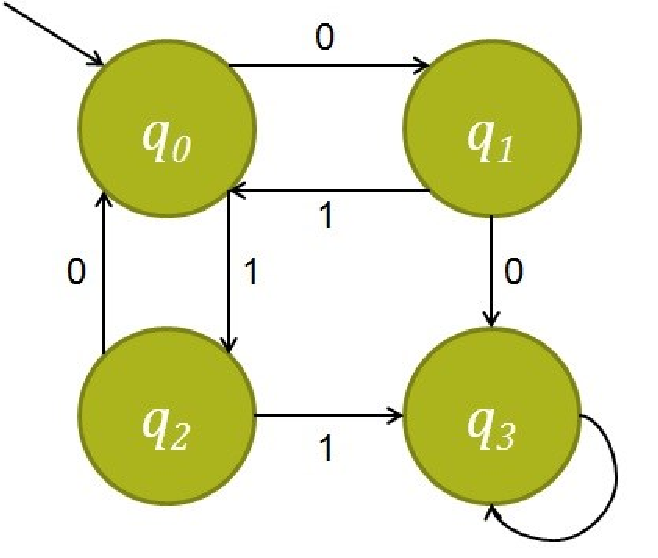
\includegraphics[width=\textwidth,height=0.8\textheight,keepaspectratio]{example-crop}
\end{minipage}}
%\vspace{-0.5em}
\caption{Requirements and possible implementation for example}
%\vspace{-1.5em}
\label{fg:example}
\end{figure}

The left side of Fig.~\ref{fg:example} shows a (somewhat contrived) contract for a system that detects whether a string of two zeros or two ones ever occurs in a stream of inputs written in a dialect of the Lustre language~\cite{lustrev6}.  The right side shows a possible implementation of that contract, visualized as a state machine.
%
Rather than use this implementation, we would like to synthesize a new one directly from the contract. There are two unassigned variables in the contract,
\texttt{x} and \texttt{state}.
The \texttt{{-}{-}\%REALIZABLE} statement specifies that \texttt{x} is a system
input, and by its absence, that \texttt{state} is a system output. The contract's 
assumption is specified by the \texttt{assert} statement and restricts the allowable input values of \texttt{x} to either 0 or 1. We also have five guarantees:
\texttt{guarantee2} and \texttt{guarantee3} are used to indirectly
describe some possible transitions in the automaton;\footnote{In Lustre, the
arrow (\texttt{->}) and \texttt{pre} operators are used to provide an initial value and access the previous value of a stream, respectively.} \texttt{guarantee5} specifies the range of
values of variable \texttt{state};
\texttt{guarantee1} and \texttt{guarantee4} are the requirements with respect to
two local variables, \texttt{bias} and \texttt{bias\char`_max}, where
 \texttt{bias} calculates the number of successive ones or
zeros read by the automaton and \texttt{bias\char`_max} indicates that at least two zeros or two ones have been read in a row.

Note that while Lustre is a compilable language, using standard compilation tools the ``program'' in Fig.~\ref{fg:example} would not compile into a meaningful implementation: it has no outputs!  Instead, it defines the guarantees we wish to enforce within the controller, and our synthesis tool will construct a program which meets the guarantees.

The realizability check on this example succeeds with a k-inductive
proof of length $k = 1$. The two corresponding
$\forall\exists$-formulas ($k=0$ for the base check and $k=1$ for the
inductive check) are valid, and thus \aeval extracts two witnessing
Skolem functions that effectively describe assignments to the local
variables of the specification, as well as to \texttt{state} (see
Appendix~\ref{app:ex} for the particular formulas).

The Skolem functions are used to construct the final implementation
following the outline provided in Template~\ref{alg:synt}.
The main idea is to redefine each variable in the model
as an array of size equal to $k$ and
to use the $k$-th element of each array as the corresponding output of the call
to $k$-th Skolem function. After this initialization process, we use an infinite
loop to assign new values to the element corresponding to the last Skolem
function, to cover the inductive step of the original proof. The final code, a
snippet of which is presented below, is 144 lines long.
Since each Skolem is represented by an $\mathit{ite}$-statement (to be explained
in Sect.~\ref{sec:aeval}), each branch is further encoded into a C-code, as
shown in Figure~\ref{fg:snippet}.

\begin{figure}[t!]
%\begin{framed}
\vspace{-2em}
\begin{minipage}{2.0\textwidth}
\begin{lstlisting}[basicstyle=\scriptsize,language=C]{Name=test2}
if (((x[1] == 1 && (-1 == bias[0])) || (x[1] == 0 && (1 == bias[0])))
     && !bias_max[0] && (state[0] != 0 || x[1] == 0)
     && (!state[0] != 0 || x[1] == 1)) {
  bias_max[1] = 0;
  bias[1] = 0;
  state[1] = 0;
}
\end{lstlisting}%
\end{minipage}
%\end{framed}
\vspace{-1em}
\caption{A code snippet of the synthesized implementation for the contract from Fig.~\ref{fg:example}.}
\vspace{-.5em}
\label{fg:snippet}
\end{figure}%

Notice how each variable is represented by an array in the snippet above.
We chose to use this easy to understand representation in order to effectively
store all the past $k-1$ values of each variable, that may be needed during the
construction of the k-inductive proof.

Recall that the user-defined model explicitly specifies only two transitions
(via \texttt{guarantee2} and \texttt{guarantee3}), while the set of implicitly defined transitions (via \texttt{guarantee1} and \texttt{guarantee4}) is incomplete.
%For example, the model does not specify an incoming transition to (\texttt{state = 0}).
Interestingly, our synthesized implementation turns all implicit transitions
into explicit ones which makes them executable and, furthermore, adds the
missing ones (e.g., as in the aforementioned snippet, from \texttt{state = 1} to \texttt{state = 0}).
\fi